\documentclass{beamer}                             % presentation
% \documentclass[draft]{beamer}                    % improves compile time
% 36x24 inch poster
\usepackage[orientation=landscape,size=custom,width=91.44,height=60.96,scale=1,debug]{beamerposter}
\usepackage[utf8]{inputenc}                        % utf8
\usepackage[T1]{fontenc}                           % fix font encoding
\usepackage[english]{babel}                        % language
\usepackage{geometry, hyperref, fancyhdr, algorithm}
\usepackage{amsmath, amssymb, amsthm}              % ams mathematical packages
\usepackage{physics, mathtools, bm}                % extra math packages
\usepackage[font=small]{subcaption}
\usepackage{graphicx, wrapfig}                     % images
\usepackage{fvextra, textcomp, CJKutf8}            % misc. text formatting
\usepackage[autostyle, english=american]{csquotes} % quotes
\usepackage{tikz, pgfplots, tikz-network}          % plots and graphs
\usepackage[noend]{algpseudocode}                  % algorithm psuedocode
\usepackage[cache=true]{minted}                    % source code
\usepackage[style=ieee]{biblatex}                  % bibliography

\pgfplotsset{compat=1.17}                          % version of pgfplots

\hypersetup{
  colorlinks=true,
  urlcolor=cyan,
  linkcolor=magenta
}

\setminted[]{
  linenos=false,
  breaklines=true,
  encoding=utf8,
  fontsize=\normalsize,
  frame=lines,
  framesep=2mm
}

% https://tex.stackexchange.com/questions/343494/minted-red-box-around-greek-characters
\makeatletter
\AtBeginEnvironment{minted}{\dontdofcolorbox}
\def\dontdofcolorbox{\renewcommand\fcolorbox[4][]{##4}}
\makeatother

\graphicspath{{./images/}}

\def\bibfont{\scriptsize}
\addbibresource{ref.bib}

\usetheme{Pittsburgh}
\usecolortheme{whale}
% hide navigation buttons
\setbeamertemplate{navigation symbols}{}
% number figures
\setbeamertemplate{caption}[numbered]

% title page
\title[]{\huge manGANime: Future Video Prediction with Conditional GANs}
\subtitle{}
\author[Huan, Thistlethwaite]{\Large Stephen Huan, Luke Thistlethwaite}
\institute[TJHSST]
{
  \large TJHSST Computer Systems Lab, 2020--2021
}
\date[]{}
\titlegraphic{\vspace{-20mm}} % remove date space
\subject{Computer Science}

\begin{document}

\begin{frame}
  \maketitle
  \begin{columns}

    %%% column 1

    \begin{column}{0.33\textwidth}
      \begin{block}{Introduction} \label{sec:intro}  
        \setlength{\parindent}{1em}
          A class of neural networks called generative adversarial networks
          (GANs) are now able to generate images of astounding quality and
          resolution \cite{stylegan, stylegan2, stylegan2ada}. However,
          these successes in unsupervised \emph{image} generation have not
          necessarily translated to \emph{video} generation \cite{dvdgan}.
          Motivated by these shortcomings, we propose replacing the real
          world with the simplified domain of cartoon video produced in
          Japan, or \emph{anime}.

          Our reasons for focusing on anime are multifaceted: first, there
          is a large volume of unlabeled anime on the internet. Secondly,
          many assumptions existing algorithms \cite{dvdgan, scene} make are
          justified in anime \textit{a priori}, but not necessarily in the
          real world. Finally, there is a huge demand for anime but a shortage
          of labor, causing animators to work long hours for low pay. Machine
          learning systems like the ones already used by Sony can automate
          tedious work, allowing animators to focus on the creative aspects.

          However, anime is not so abstract as to destroy any
          semblance of the real world. For example, the object
          detection model YOLOv4 can be directly applied to anime.

          \begin{figure}[h!]
            \centering
            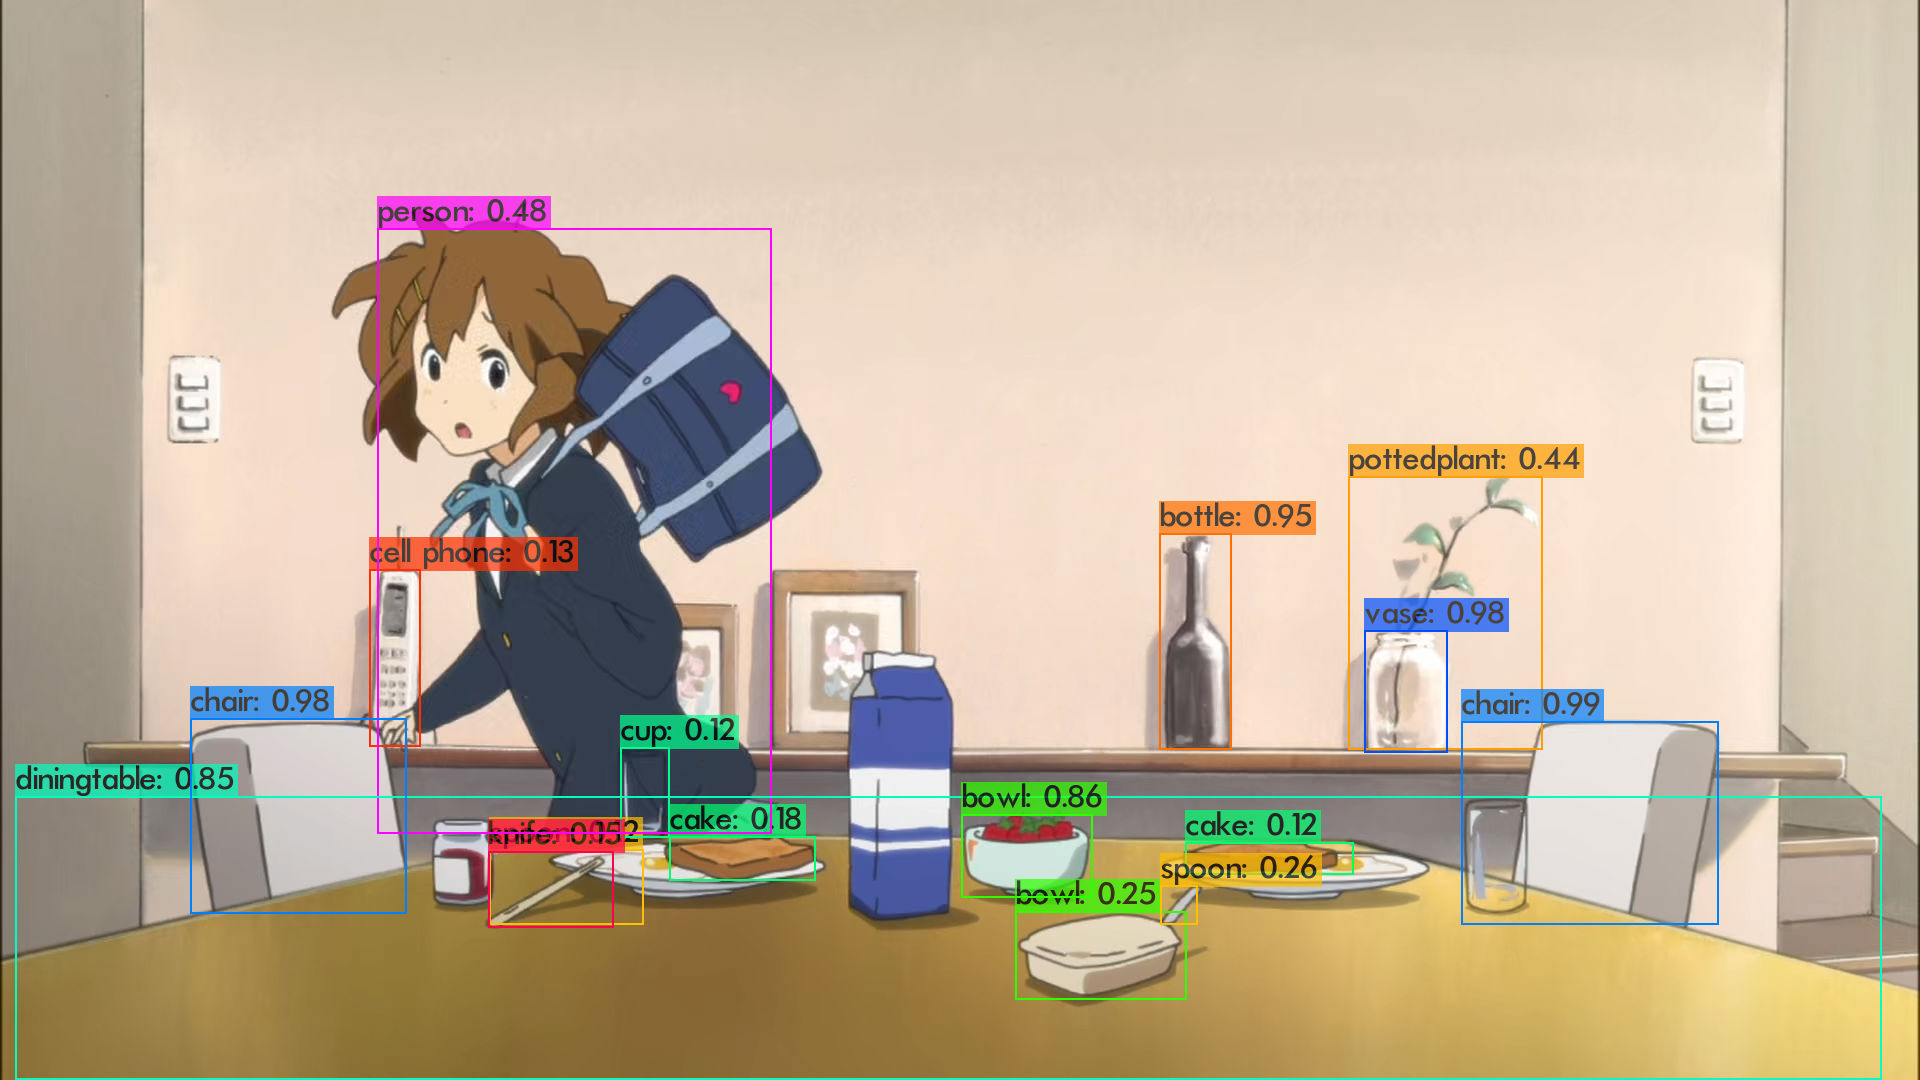
\includegraphics[scale=0.4,trim={0 0 0 190px},clip]{yolov4}
            \caption{YOLOv4-CSP on the anime \textit{K-On!}. See
              \href{https://youtu.be/i8jCzh9nWc4}{https://youtu.be/i8jCzh9nWc4}
              for a demonstration.}
            \label{fig:object}
          \end{figure}

          Animation is expensive, so anime is often produced with reference
          to a comic book, or \textit{manga}. Certain anime will follow their
          source very precisely, as shown in Figure \autoref{fig:dual}.

          \begin{figure}[h!]
              \centering
              \begin{subfigure}[h]{0.49 \textwidth}
                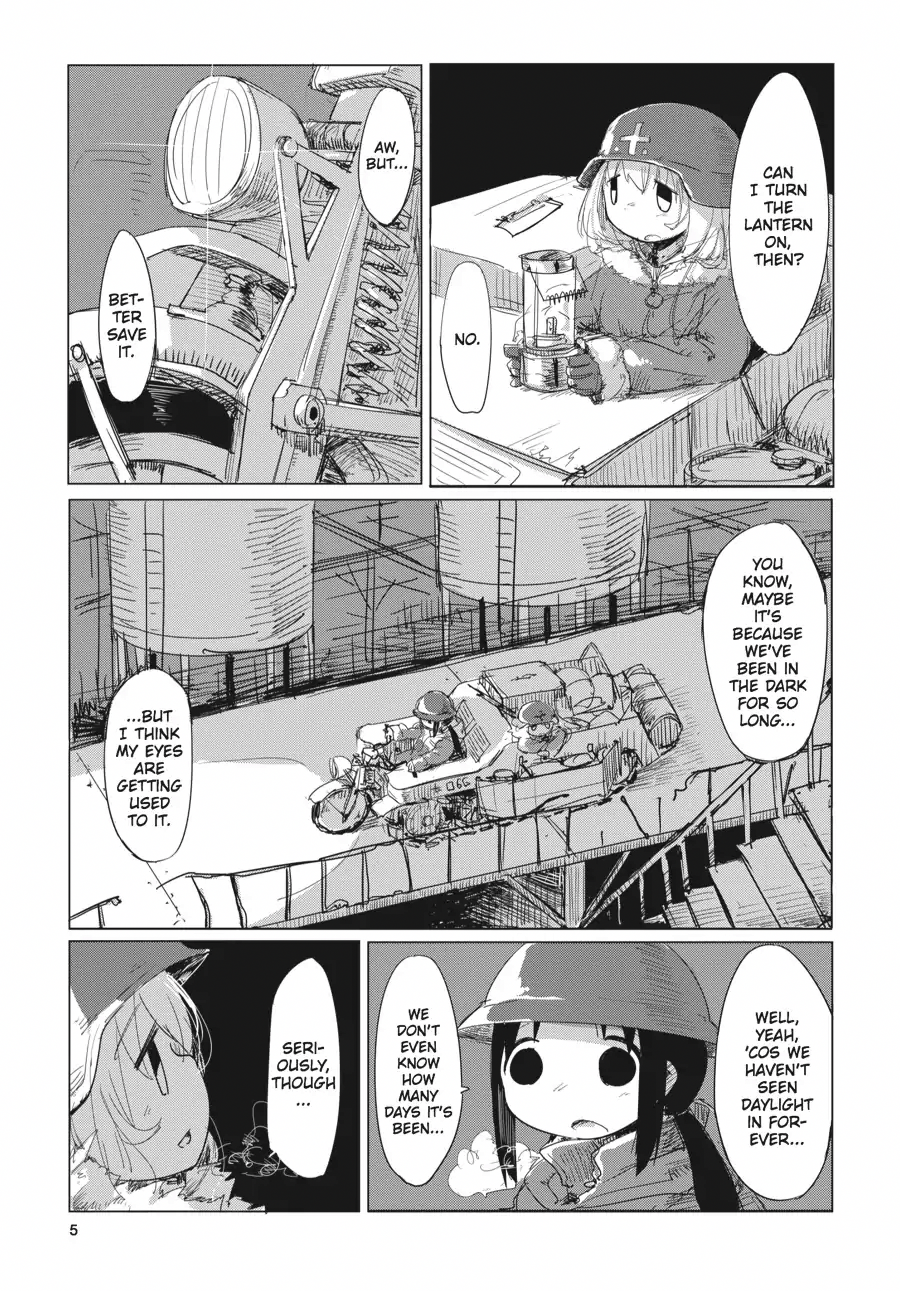
\includegraphics[scale=0.3,trim={60px 50px 60px 60px},clip]{page}
                % \caption{A manga page from \textit{Girls' Last Tour}.}
              \end{subfigure}
              \hfill
              \begin{subfigure}[h]{0.49 \textwidth}
                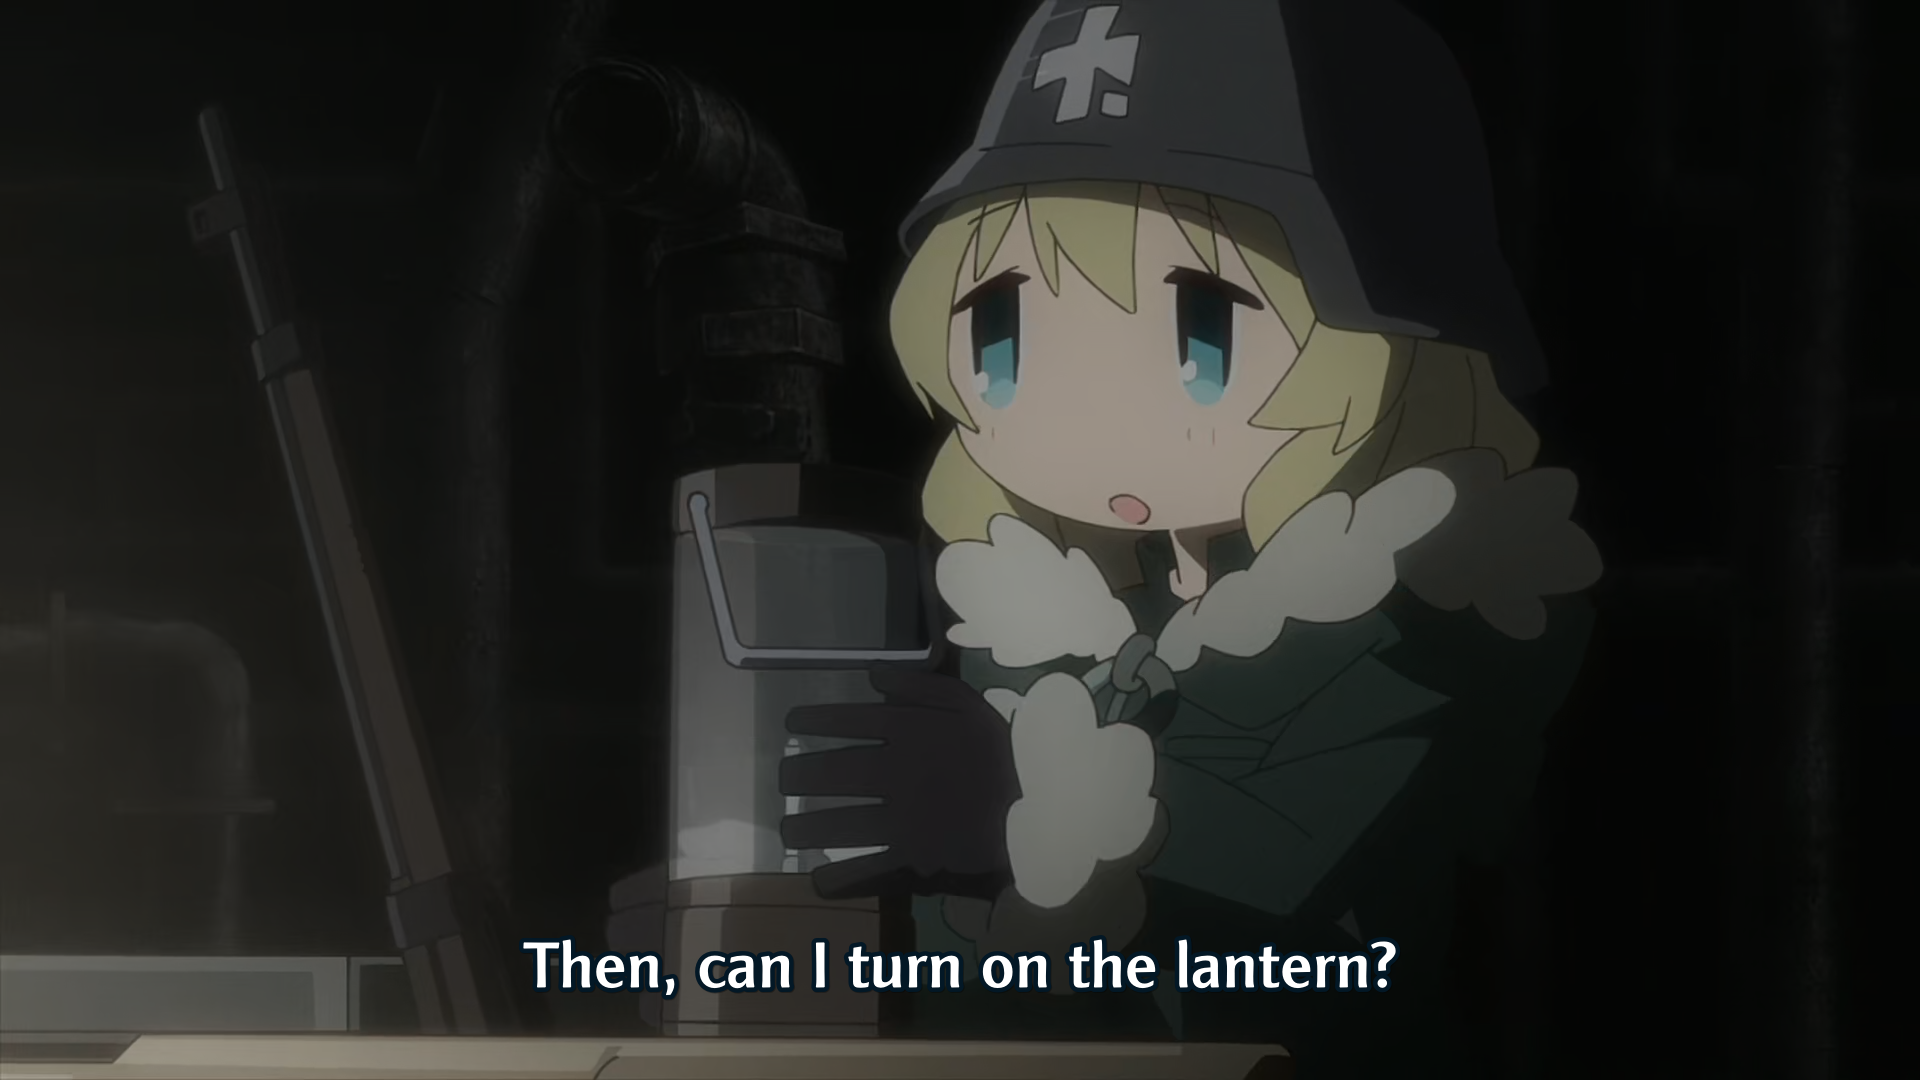
\includegraphics[scale=0.28,trim={160px 0 300px 0},clip]{frame}
                % \caption{A anime frame from \textit{Girls' Last Tour}.}
              \end{subfigure} 
              \caption{The high correspondence between manga (left)
                and anime (right) in \textit{Girls' Last Tour}.}
              \label{fig:dual}
          \end{figure}

        For manga to be a useful conditioning signal, it should correspond well
        with its anime. Formally speaking, we define a \textit{page function}
        \( f: \mathbb{Z} \to \mathbb{Z} \) that maps an anime frame index to
        its corresponding manga page. The existence of \( f \) implies each
        frame is mapped, so we remove frames without support, for example,
        \enquote{intro} and \enquote{outro} songs. We further enforce that \( f
        \) is monotonic, i.e. \( x \leq y \) implies \( f(x) \leq f(y) \). 

      \end{block}

    \end{column}

    %%% column 2

    \begin{column}{0.33\textwidth}
      \begin{block}{Making a Dataset}
        \setlength{\parindent}{1em}
        \begin{wrapfigure}{r}{0.5\textwidth}
          \centering
          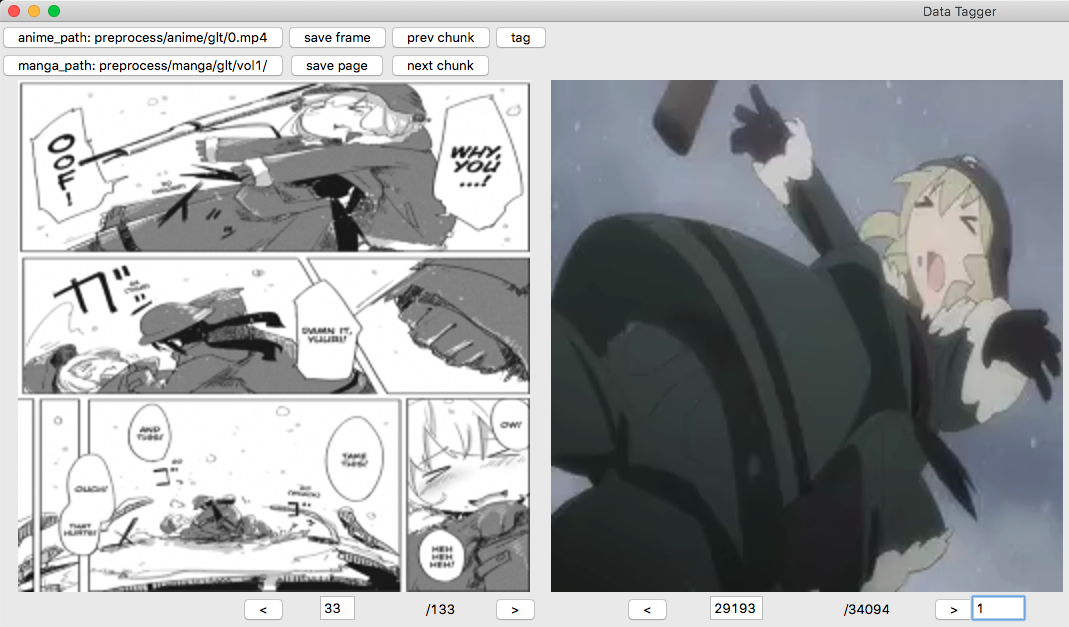
\includegraphics[scale=0.4]{data_tagger}
          \caption{GUI for efficient manual data tagging.}
          \label{fig:tag}
        \end{wrapfigure}

        In order to construct \( f \) we tag each frame of the anime with
        its corresponding manga page. There are 174,792 total frames for
        \textit{Girls' Last Tour} and 533 manga pages, which is too much
        to label by hand. But because \( f \) is monotonic, the anime
        \enquote{goes in the same order} as the manga; we only need to tag
        the \textit{boundaries} when \( f \) changes. This is implemented in
        a graphical user interface (GUI) shown in Figure \autoref{fig:tag}.
        However, we still need to find which frames mark a transition between
        manga pages, which can be detected by measuring if the similarity
        between adjacent frames is less than a certain cutoff.

        We generalize the dot product similarity to the element-wise
        product of two tensors. Our similarity is then \( \rho(A, B)
        = \frac{A \cdot B}{\norm{A} \norm{B}} \) where \( \norm{X} =
        \sqrt{X \cdot X} \), with a cutoff of 0.8.
      \end{block}

      \begin{block}{Methods}
        \setlength{\parindent}{1em}
        We condition an unsupervised model for video generation
        by \textit{replacing} the latent with our image data. The
        dimensionality of the latent \( \bm{z} \) is 512 while we need
        to fit two 256x256 images (initial frame and manga page), so we
        greyscale, apply a 16x16 average pool, then concatenate to form
        \( \bm{x} \). Finally, we use \( \bm{z} = 2 \bm{x} - 1 \) in
        order to center at 0. \( \bm{z} \) is passed to the generator
        \( G \), which generates videos according to the recurrence:
        \[ F_{n + 1} = G(F_n; M(n)) \]
        where \( F_n \) is the \( n \)th frame and \( M(n) \) is the page
        function defined above. \( F_0 \) is the initial conditioning frame.
        We then optimize \( G \) with mean squared loss and gradient decent.
      \end{block}
 
      \begin{block}{Latent Space Exploration}
      \setlength{\parindent}{1em}
        We first try to project an image, i.e. given an image \( X \) find
        a latent vector \( \bm{w} \) such that \( G(\bm{w}) \) is as close
        to \( X \) as possible. Next, given two latents \( \bm{w}_0 \) and
        \( \bm{w}_1 \), we can linearly interpolate between the two with \(
        \bm{w}(t) = \bm{w}_0 + t (\bm{w}_1 - \bm{w}_0) \), \( t \in [0, 1] \).
      \end{block}

      \begin{block}{Training StyleGAN2 with Adaptive Discriminator Augmentation (ADA) \cite{stylegan2ada}} 
      \setlength{\parindent}{1em}
        \begin{figure}[h!]
            \centering
            \begin{subfigure}[h]{0.49 \textwidth}
              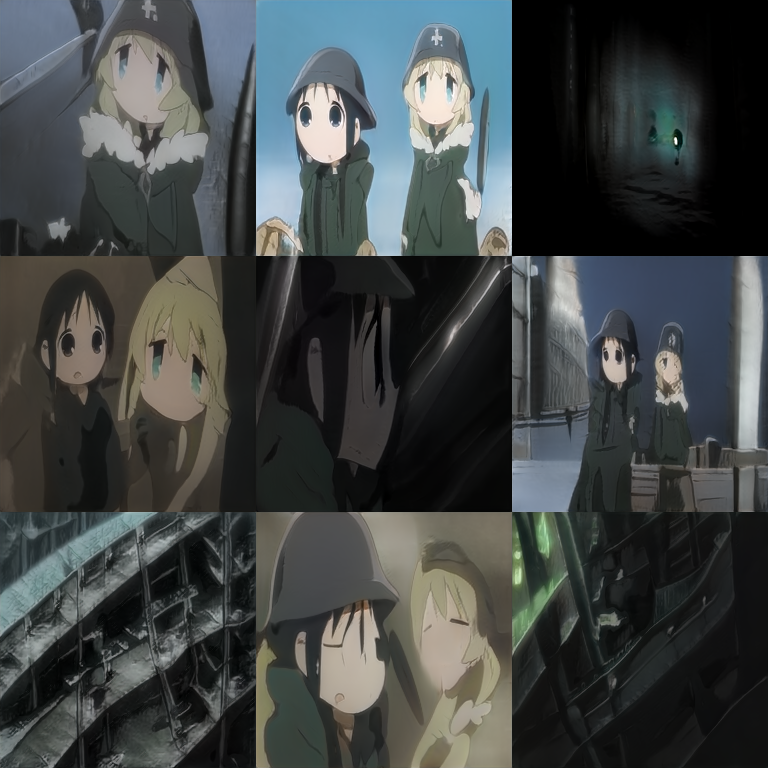
\includegraphics[scale=0.4]{samples_gan}
              % \caption{Generated images.}
            \end{subfigure}
            \hfill
            \begin{subfigure}[h]{0.49 \textwidth}
              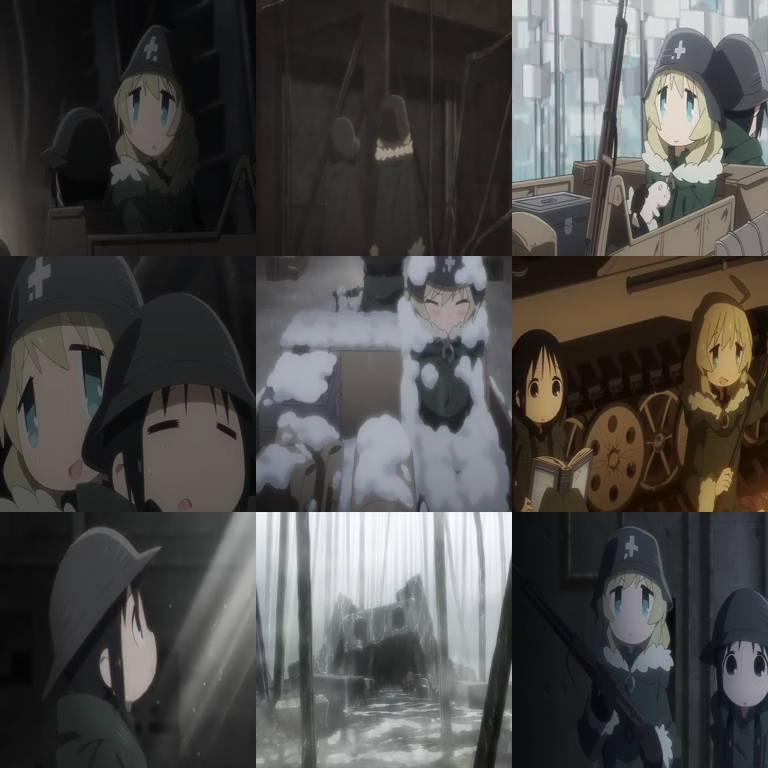
\includegraphics[scale=0.4]{samples_real}
              % \caption{Real images.}
            \end{subfigure}
            \caption{Although certain generated images (left) are strikingly
              similar to the ground truth (right) e.g. the top left of both,
              the generated images show clear distortions and are discernible
              from the real images.}
            \label{fig:samples}
        \end{figure}

        We trained StyleGAN2-ADA \cite{stylegan2ada}, achieving a Fréchet
        inception distance (FID) of 25.722. FID is a common metric of
        generated image quality; this is relatively high compared to the
        FID of 3.88 achieved on the FFHQ dataset by \cite{stylegan2ada}
        (lower is better). We suspect the high correlation between video
        frames decreases diversity, hindering training.
      \end{block}

    \end{column}

    %%% column 3

    \begin{column}{0.33\textwidth}

      \begin{block}{Conditioning StyleGAN}
      \setlength{\parindent}{1em}
        \begin{figure}[h!]
          \centering
          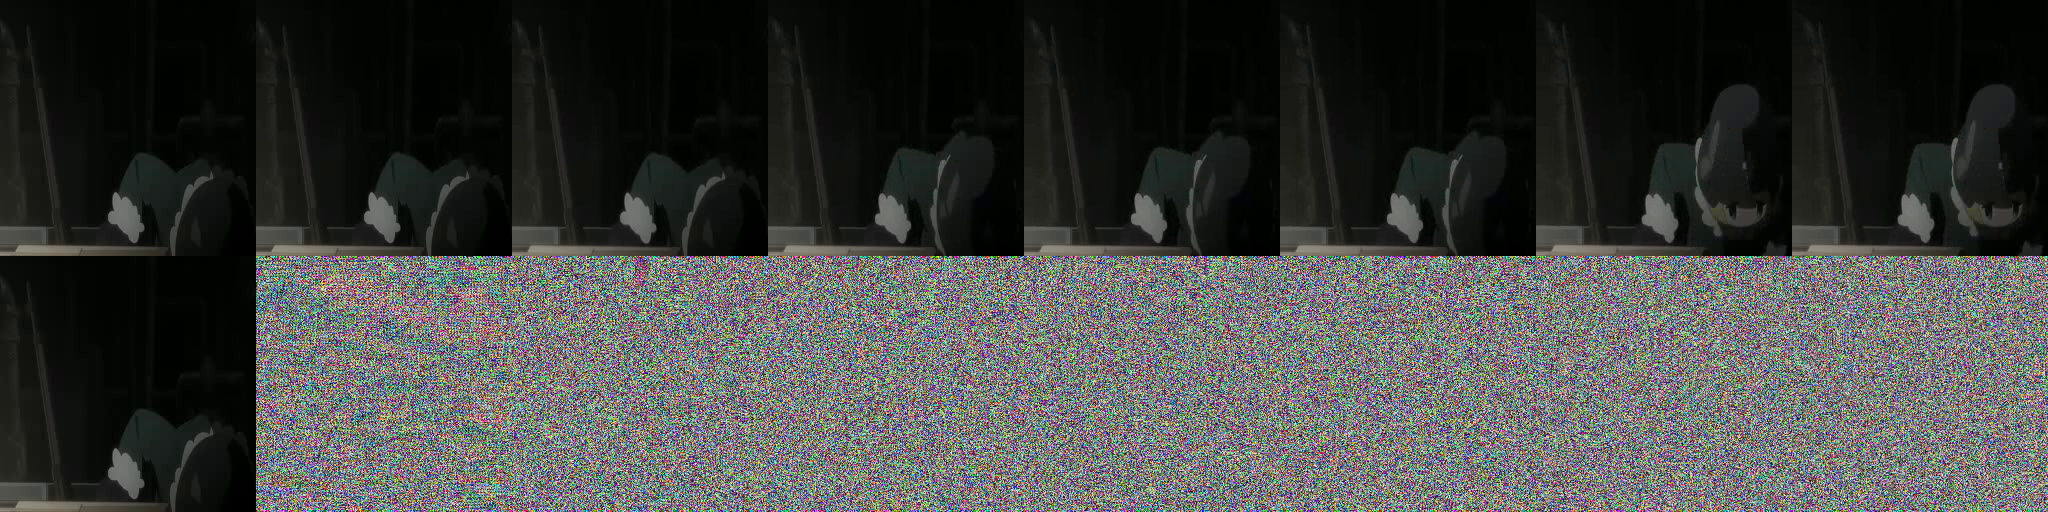
\includegraphics[scale=0.4]{results_gen}
          \caption{Top row is the ground truth and
                   the bottom row is generated output.}
          \label{fig:gen}
        \end{figure}

        We find that the generator outputs noise. We suspect a capacity issue,
        as \( \bm{z} \)'s dimensionality is too small to effectively encode the
        initial frame and manga page, so the generator loses the only benefit
        of conditioning, then is dominated by the discriminator.
       \end{block}

      \begin{block}{Latent Space Exploration}
      \setlength{\parindent}{1em}
        \begin{figure}[h!]
          \centering
          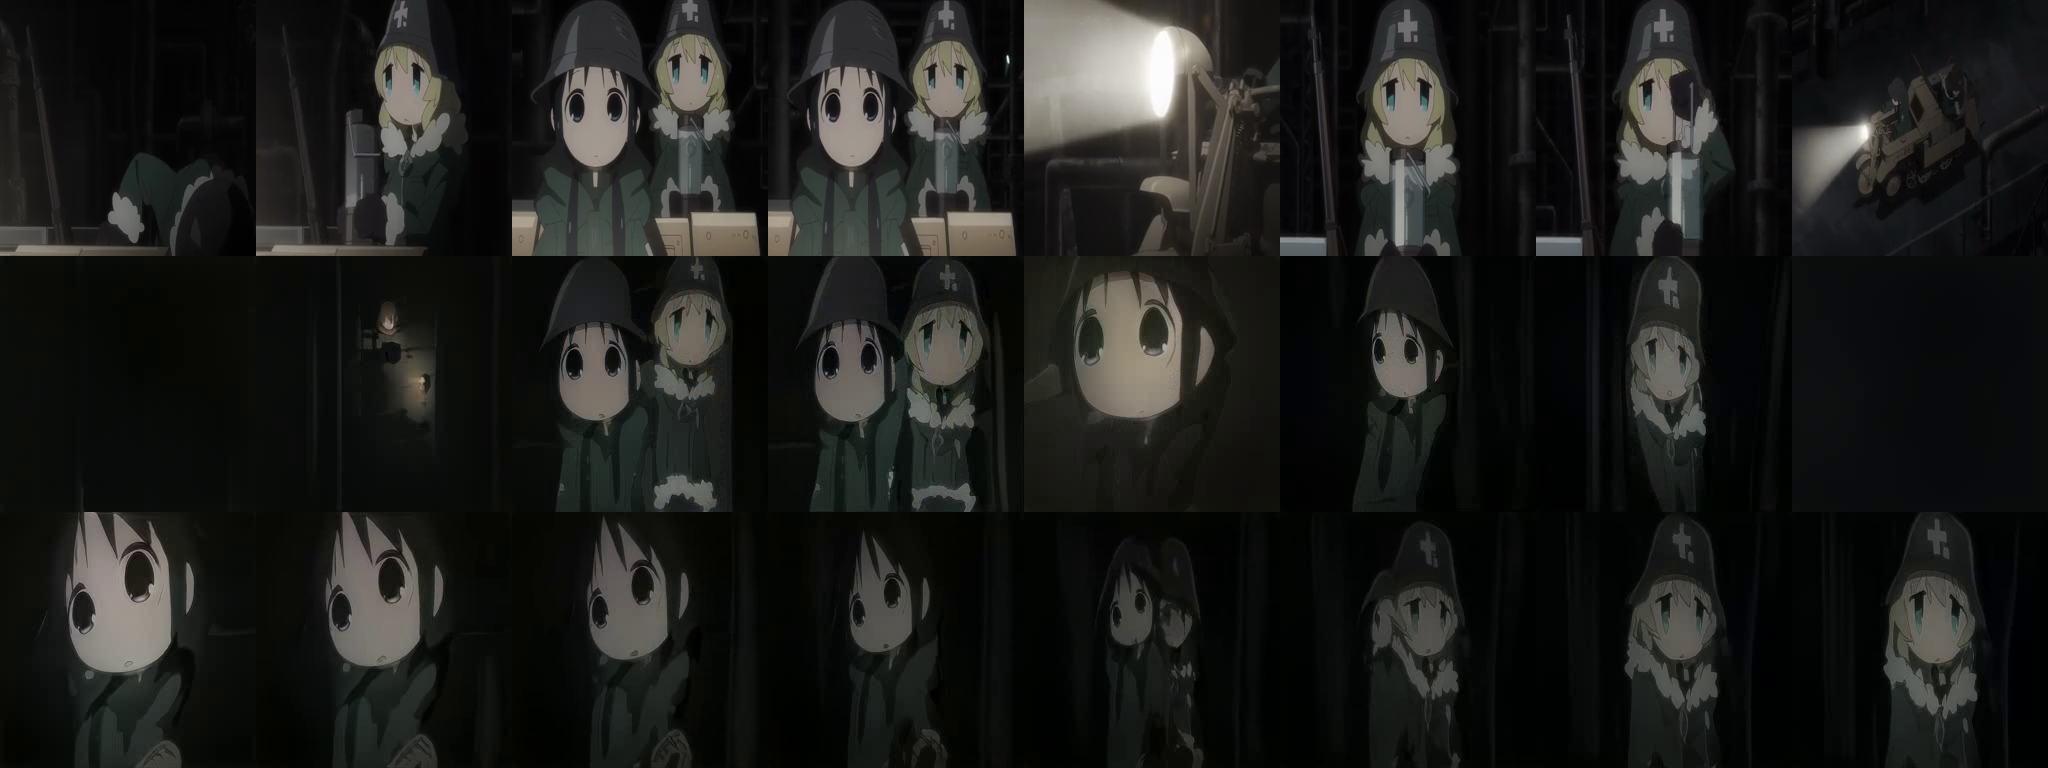
\includegraphics[scale=0.4]{results_latent}
          \caption{Top row is the ground truth, middle row is a
            projection of each frame into the latent space, and the
            bottom row is a linear interpolation. For the videos, see
            \href{https://youtu.be/4J9BBHX-uNg}{https://youtu.be/4J9BBHX-uNg}.}
          \label{fig:latent}
        \end{figure}

        For projection, frames 3, 4, and 7 are reconstructed well
        but others are not represented at all. We suspect only
        frequently occurring images can be convincingly represented.

        For linear interpolation, we find that the video is \enquote{smooth}
        since the perceptual path length metric and path length regularization
        discussed in \cite{stylegan, stylegan2} incentives smoothness by
        minimizing adjacent perceptual differences and by preserving path
        lengths.
      \end{block}

      \begin{block}{Conclusion}
      \setlength{\parindent}{1em}
        Dismayed at the state of video generation, we propose the simplified
        domain of anime. We discuss important features of anime/manga for
        creating a dataset from unlabeled video. We then experiment with
        adjusting StyleGAN \cite{stylegan2ada} for future video prediction
        with conditioning and with latent interpolation. Although our
        results are poor, we believe the avenues of research laid out in
        this work can be improved in future experiments; one approach may
        be to add a foreground/background mask \cite{scene} to DVD-GAN
        \cite{dvdgan} and then upscale with a deep super-resolution
        algorithm like \href{https://github.com/nagadomi/waifu2x}{waifu2x}
        or \href{https://github.com/akai-katto/dandere2x}{dandere2x}.
      \end{block}

      \begin{block}{References}
        \printbibliography  
      \end{block}

    \end{column}

  \end{columns}
\end{frame}
\end{document}
